\chapter{Simulation study}\label{chap:applications}
\fancyhead[LO]{\nouppercase{\leftmark}}
In this chapter, I apply the ODE-VAE model developed in Chapter~\ref{chap:methods} to different simulated data settings inspired by the scenario of the NAKO sub study outlined in Chaper~\ref{chap:intro}. First, I explain the simulation design and give details on the model implementation. 
Next, I present results from training the model on data generated from linear and non-linear two-dimensional ODE systems with two unknown parameters and on a linear system with four unknown parameters, where I employ the approach of Chapter~\ref{chap:methods}, Section~\ref{sec:methods-minibatches} to train on batches of similar individuals. I compare scenarios with different variants of simulated baseline information, with different amounts of noise present in the baseline variables, and with different noise levels in the simulated measurements of the true underlying trajectory. 

\section{Simulation design}

In all simulated data settings, two distinct underlying development patterns are modelled, each given as the solution of a two-dimensional ODE system. Thus, all observations can be categorised into two groups with distinct development patterns and there are two central components characterising each development pattern. 
Since our aim is to recover those central factors of variation as time-continuous functions in the latent representation, the VAE latent space is set to be two-dimensional. 

After specifying the general structure of the two-dimensional ODE, two sets of parameters are defined for the common underlying system structure, such that the two resulting ODE systems have qualitatively different -- and thus easily distinguishable -- solutions. For example, in a linear case, I define one system where both components display a downward trend, and the other one with an upward trend in one component and a downward trend in the other component. 

Both the linear and the non-linear ODE systems are governed by four parameters. In the applications of Sections~\ref{sec:apps-linear2p} and \ref{sec:apps-nonlinear2p}, two of these parameters are assumed as known and explicitly defined beforehand together with the general linear or Lotka-Volterra-like structure of the ODE system. During training, the model then only learns estimates for the two remaining parameters as outputs of the ODE-net. In the application of Section~\ref{sec:apps-linear4p}, all four parameters are assumed to be unknown and estimated with the ODE-net.

Generally, I simulate observations of $n$ individuals by drawing from the true underlying trajectories given as solutions of the pre-defined ODE systems with random noise to account for the measurement error. 
Individuals are randomly divided into two groups of equal size defined by the two distinctly parameterised underlying ODE systems. Algorithm~\ref{algo-simulation-time-dependent} summarises the simulation procedure. 
For each individual, two observations of $p=10$ variables are generated, one observation at a common baseline timepoint $t_0 = 0$ and one at an individual-specific second time point $t_1^i$ sampled uniformly from the interval $[1.5,10]$.
I chose $1.5$ as earliest second time point to account for the assumption that no individual was measured again directly after the basline time point. 
The simulation should reflect the assumption that the underlying development patterns form a compressed representation of the measurements and that there are groups of observed variables sharing a common trend. Thus, for each individual, measurements of the first five variables are simulated by sampling from the first component of the individual's true trajectory both at the common baseline time point $t_0$ and at the individual-specific second time point $t_1^i$. For variables $6$ to $10$, I sample in the same fashion from the second component of the individual's true trajectory at both time points. 
Specifically, for each time point, I draw a variable-specific measurement error $\delta_{j}\tn, \delta_{j}\te \sim \mathcal{N}(0,\sigma_{\mathrm{var}}^2)$ for $j=1,\dots, p=10$ and an individual-specific measurement error $\varepsilon_{i,j}\tn, \varepsilon_{i,j}\te \sim \mathcal{N}(0,\sigma_{\mathrm{ind}}^2)$ for $i=1,\dots, n$, $j=1,\dots, p$ and add them to the true value of the corresponding component of the ODE solution at $t_0$ and $t_1^i$, respectively. 
The standard deviations $\sigma_{\mathrm{var}}$ and $\sigma_{\mathrm{ind}}$ of the measurement error distributions determine the level of noise in the data. 
\begin{algorithm}
	\SetAlgoLined
	\KwData{$n\in 2\cdot\N,~~p\in \N,~~\sigma_{\mathrm{var}}, \sigma_{\mathrm{ind}} \in \R^+$}
	\KwResult{%dataset 
		$\mathcal{D} = \lbrace x_1,\dots, x_n\rbrace$ 
		with $x_i = (x_i\tn, x_i\te), i=1,\dots, n$}
	\textbf{Initialise:} 
	sample random permutation $\pi({1,\dots, n})$ and set $\mathrm{group}_1 = \lbrace\pi({1,\dots, n})_k \mid k=1,\dots, \frac{n}{2}\rbrace$, $\mathrm{group}_2 = \lbrace\pi({1,\dots, n})_k \mid k=(\frac{n}{2}+1),\dots, n\rbrace$\; 
	\For{$j=1,\dots, p=10$}{
		sample $\delta_{j}^{t_0},~\delta_{j}^{t_1} \sim \mathcal{N}(0,\sigma_{\mathrm{var}}^2)$\;}
	\For{$i=1,\dots, n$}{
			sample $t_i^1 \sim \mathrm{UC}_{\left[1.5,10\right]}$\;
			solve $v_1^{t_i^1} = \mathrm{ODEsolve}(f_{\mathrm{group}_i}(u_1,t),u_1(t_0),t_i^1)$, $v_2^{t_i^1} = \mathrm{ODEsolve}(f_{\mathrm{group}_i}(u_2,t),u_2(t_0),t_i^1)$\;
		\For{$j=1,\dots, \frac{p}{2}$}{
			sample $\varepsilon_{i,j}^{t_0},~ \varepsilon_{i,j}^{t_1} \sim \mathcal{N}(0,\sigma_{\mathrm{ind}}^2)$\;
			compute $x_{i,j}^{t_0} = u_1(t_0) + \delta_{j}^{t_0} + \varepsilon_{i,j}^{t_0}$,
			$x_{i,j}^{t_1} = v_1^{t_i^1} + \delta_{j}^{t_1} + \varepsilon_{i,j}^{t_1}$\;}
		\For{$j=(\frac{p}{2}+1),\dots, p$}{
			sample $\varepsilon_{i,j}^{t_0},~ \varepsilon_{i,j}^{t_1} \sim \mathcal{N}(0,\sigma_{\mathrm{ind}}^2)$\;
			compute $x_{i,j}^{t_0} = u_2(t_0) + \delta_{j}^{t_0} + \varepsilon_{i,j}^{t_0}$,
			$x_{i,j}^{t_1} = v_2^{t_i^1} + \delta_{j}^{t_1} + \varepsilon_{i,j}^{t_1}$\;}		
	}
	\caption{Simulation of time-dependent variables}
	\label{algo-simulation-time-dependent}
\end{algorithm}

In addition to the time-dependent variables, I simulate measurements of $q=50$ additional baseline variables representing the individuals' more extensive characterisation that are assumed to be potentially informative about the individual development pattern in the time-dependent variables (see Chapter~\ref{chap:methods}, Section~\ref{sec:methods-ODEparamswithbaselineinfo}).

Here, two different approaches are applied as summarised in Algorithms~\ref{algo-simulation-baseline-trueODEparams} and \ref{algo-simulation-baseline-groupinfo}. In the first version, the values of the baseline variables are drawn from the individual's true ODE parameters with random noise. For each unknown ODE parameter, I simulate a number of variables containing noisy values of this one ODE parameter and add noise variables not containing any information, such that I end up with a total of $50$ baseline variables.  
In Section~\ref{sec:apps-nonlinear2p-diffbaselinenumbers}, I discuss the effect of changing the number of noise variables and present results for different settings. 

The second version models a scenario where only some knowledge about the group membership of each individual is assumed. 
We can imagine to know that the observed individuals can be classified into two groups that are expected to exhibit different development patterns. As an example, if the time-dependent variables measure lung functions and there are smoking and non-smoking individuals in the dataset, it can be assumed that the general development of lung functionality for smoking people will differ from that of non-smokers and we can use that information to estimate individual-specific ODE parameter sets. 
Again, I simulate a number of variables with values sampled from the individual's group membership (encoded as $+1$ or $-1$) with random noise and add noise variables as in the first version of simulated baseline variables with the true ODE parameters. 
The number of baseline variables containing information either about the true ODE parameters or the group membership is denoted with $q_{\mathrm{info}}$. 
\begin{algorithm}
	\SetAlgoLined
	\KwData{$n\in 2\N,~~q, q_{\mathrm{info}}\in\N,~~\sigma_{\mathrm{info}}, \sigma_{\mathrm{noise}}\in \R^+$}
	\KwResult{
		$\lbrace y_1,\dots, y_n\rbrace$ 
		with $y_i = (y_{i,1}, \dots, y_{i,q})^{\top}, i=1,\dots, n$}
	\For{$j=1,\dots, q_{\mathrm{info}}$}{
		\For{$i=1,\dots, n$}{
		sample $y_{i,j} \sim \mathcal{N}(\mathrm{ODEparameters}_{\mathrm{group_i}},\sigma_{\mathrm{info}}^2)$\;}
	}
	\For{$j=(q_{\mathrm{info}}+1),\dots, q$}{
		\For{$i=1,\dots, n$}{
		sample $y_{i,j} \sim \mathcal{N}(0,\sigma_{\mathrm{noise}}^2)$\;}
	}
	\caption{Simulation of baseline variables with true ODE parameters}
	\label{algo-simulation-baseline-trueODEparams}
\end{algorithm}

\begin{algorithm}
	\SetAlgoLined
	\KwData{$n\in 2\N,~~q, q_{\mathrm{info}}\in\N,~~\sigma_{\mathrm{info}}, \sigma_{\mathrm{noise}}\in \R^+$}
	\KwResult{%dataset 
		$\lbrace y_1,\dots, y_n\rbrace$ 
		with $y_i = (y_{i,1}, \dots, y_{i,q})^{\top}, i=1,\dots, n$}
	\For{$j=1,\dots, q_{\mathrm{info}}$}{
		\For{$i=1,\dots, n$}{
			sample $y_{i,j} \sim \mathcal{N}(\pm 1_{\mathrm{group}_i},\sigma_{\mathrm{info}}^2)$\;}
	}
	\For{$j=(q_{\mathrm{info}}+1),\dots, q$}{
		\For{$i=1,\dots, n$}{
			sample $y_{i,j} \sim \mathcal{N}(0,\sigma_{\mathrm{noise}}^2)$\;}
	}
	\caption{Simulation of baseline variables with group membership}
	\label{algo-simulation-baseline-groupinfo}
\end{algorithm}

\section{Implementation details}\label{sec:apps-implementation}

The following section provides details on the implementation of the proposed method. 
The code to run all simulations and produce all figures of this chapter is written in the Julia programming language of version 1.1.1 with the additional packages DataFrames.jl (v0.20.0), DiffEqFlux.jl (v0.10.0), DifferentialEquations.jl (v6.9.0), Distributions.jl (v0.21.9), Flux.jl (v0.9.0), LaTeXStrings.jl (v1.0.3), Plots.jl (v0.28.4), StatsBase.jl (v0.32.0) and VegaLite.jl (v1.0.0). 

For the VAE model, I aimed at keeping the architecture simple and close to established models from literature. Specifically, I used one hidden layer with the number of hidden units equal to the number of input dimensions (i.e., $10$ in all applications) and a $\tanh$-activation function shifted by $+1$. 
The latent space is set to be two-dimensional and the latent space mean and variance are obtained as affine linear transformations of the hidden layer values without a non-linear activation. The decoder includes one hidden layer with $10$ hidden units and a $\tanh$-activation function and outputs mean and variance of a Gaussian distribution that are calculated from the hidden layer by using an affine linear transformation without activation function. 
In the loss function, the KL-divergence between the prior and posterior is downweighed with a factor of $0.5$ to reduce the regularising effect. The sum of squared values of all decoder parameters with a weighting factor of $0.01$ is added as commonly used penalty term to prevent exploding model parameters. 

The ODE-net consists of three layers in addition to the input layer, two hidden layers and one output layer. In the first hidden layer, the number of units equals the number of input dimensions (i.e., $50$ in all the applications) and a $\tanh$-activation function is used. In the second layer, the number of hidden units equals the number of parameters to be estimated and the activation function is a shifted sigmoid function. The shifting of the activation function serves as a prior to guide the model in identifying the range in which to estimate the ODE parameters: For the applications with a linear underlying ODE systems and true parameters of around $0.2$ or $-0.2$ (Sections~\ref{sec:apps-linear2p} and \ref{sec:apps-linear4p}), the sigmoid function is shifted by $-0.5$ such that it outputs values in the interval $[-0.5,0.5]$. For the application on a non-linear systems with true parameters between $0.5$ and $2$, it is shifted by $+1$, such that it outputs values in $[0,2]$. However, in order not to restrict the model to those ranges but let it freely shift and scale the sigmoid-transformed values, an affine linear transformation with a diagonal matrix is added as final output layer. 

All reported numbers of epochs and learning rates are chosen based on monitoring convergence of the loss function and visualising training results. Neither a systematic grid search nor excessive tuning of these hyperparameters was performed.

For the applications with the non-linear ODE system from Section~\ref{sec:apps-nonlinear2p}, I frequently observed training runs where the random weight initialisation of the network produced instabilities in the numerical solving of the ODE with the Tsit5-ODE solver implementing a Tsitouras 5/4 Runge-Kutta method. To reduce the number of resulting training break-offs, I changed the default initialisation method for the weights to sampling from smaller values. While this did result in less solver instabilities, it did not prevent them completely.

Generally, backpropagating through the ODE solving step within the neural network framework is realised by the DiffEqFlux.jl-package (for details, see \cite{Rackauckas2019}). 

In the scenario with four unknown ODE parameters, I employed a discretisation to efficiently approximate the $L^2$-norm to determine the distance matrix (see Equation~\ref{eq:discretisationl2norm} in Chapter~\ref{chap:methods}, Section~\ref{sec:methods-batches-EMprocedure}) with $m+1=11$ equidistant values. Here, as an additional centralising step, from each value the mean of all $m+1$ values from the discretisation is subtracted to ensure the distance is based on the actual development over the time interval, not on random similarity of absolute values due to the neccessary discretisation.

\section{Linear ODE system with two unknown parameters}\label{sec:apps-linear2p}

\subsection{Structure of input data}\label{sec:apps-linear2p-inputdata}

First, two distinct underlying development patterns are defined as solutions of the two ODE systems given in Equations (\ref{eq:ODE-systems-2ps-linear1}) and (\ref{eq:ODE-systems-2ps-linear2}) and visualised in Figure~\ref{fig:true_solution_linear_2ps}. The simulated individuals fall into two groups, one with an upward trend in one component and a downward trend in the other component, and the other group with a downward trend in both components. 

\begin{figure}
	\centering
	\begin{minipage}{.5\linewidth}
		\centering
		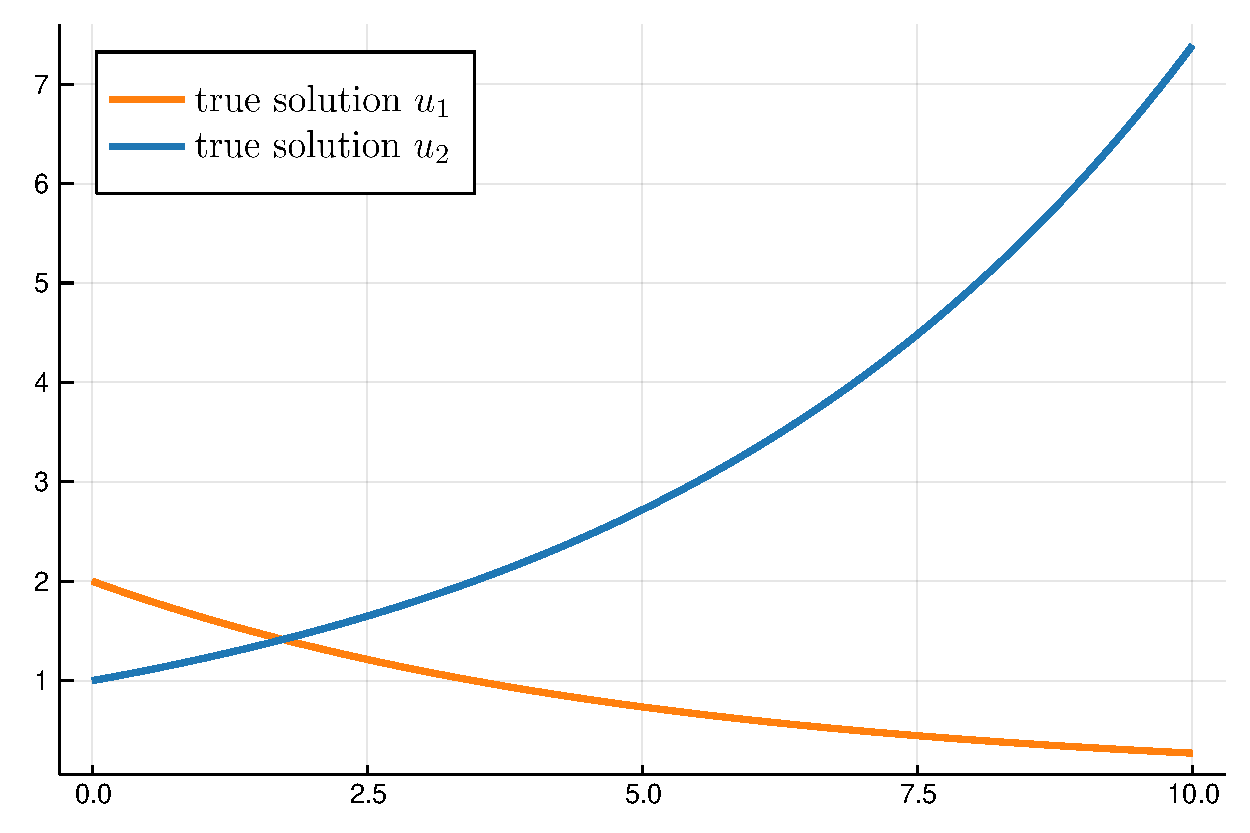
\includegraphics[width=\linewidth]{true_solution_2_2ps_linear.pdf}
		\scriptsize
		\begin{equation}\label{eq:ODE-systems-2ps-linear1}
		\begin{split}
		\frac{d}{dt}\begin{pmatrix} u_1 \\ u_2 \end{pmatrix}(t) &= \begin{pmatrix} -0.2 & 0 \\ 0 & 0.2 \end{pmatrix} \begin{pmatrix} u_1 \\ u_2 \end{pmatrix}(t); \\
		\begin{pmatrix} u_1 \\ u_2 \end{pmatrix}(0) &= \begin{pmatrix} 2 \\ 1 \end{pmatrix}
		\end{split}
		\end{equation}
		\normalsize
	\end{minipage}\begin{minipage}{.5\linewidth}
		\centering
		\includegraphics[width=\linewidth]{true_solution_1_2ps_linear.pdf}
		\scriptsize		
		\begin{equation}\label{eq:ODE-systems-2ps-linear2}
		\begin{split}
			\frac{d}{dt}\begin{pmatrix} u_1 \\ u_2 \end{pmatrix}(t) &= \begin{pmatrix} -0.2 & 0 \\ 0 & -0.2 \end{pmatrix} \begin{pmatrix} u_1 \\ u_2 \end{pmatrix}(t); \\
			\begin{pmatrix} u_1 \\ u_2 \end{pmatrix}(0) &= \begin{pmatrix} 2 \\ 1 \end{pmatrix}
		\end{split}
		\end{equation}
		\normalsize
	\end{minipage}
	\caption{True underlying development patterns characterised as solutions of two-dimensional linear ODE systems.}
	\label{fig:true_solution_linear_2ps}
\end{figure}

The data is simulated by drawing measurement points from these true trajectories with random noise as described in Algorithm~\ref{algo-simulation-time-dependent}. More precisely, I generate observations of $100$ individuals, $50$ from each of the two groups, and generate observations of $10$ variables by adding variable-specific and the individual-specific measurement errors to $5$ values from each of the two ODE solution components both at the initial time point $t_0 = 0$ and an individual-specific second time point $t_1^i$. In this first setting, I simulate a low level of noise and set $\sigma_{\mathrm{var}} = \sigma_{\mathrm{ind}} = 0.1$. Figure~\ref{fig:data_truesolution_linear2ps} visualises all simulated observations together with the true ODE solutions.
\begin{figure}
	\centering
	\begin{minipage}{.5\linewidth}
		\centering
		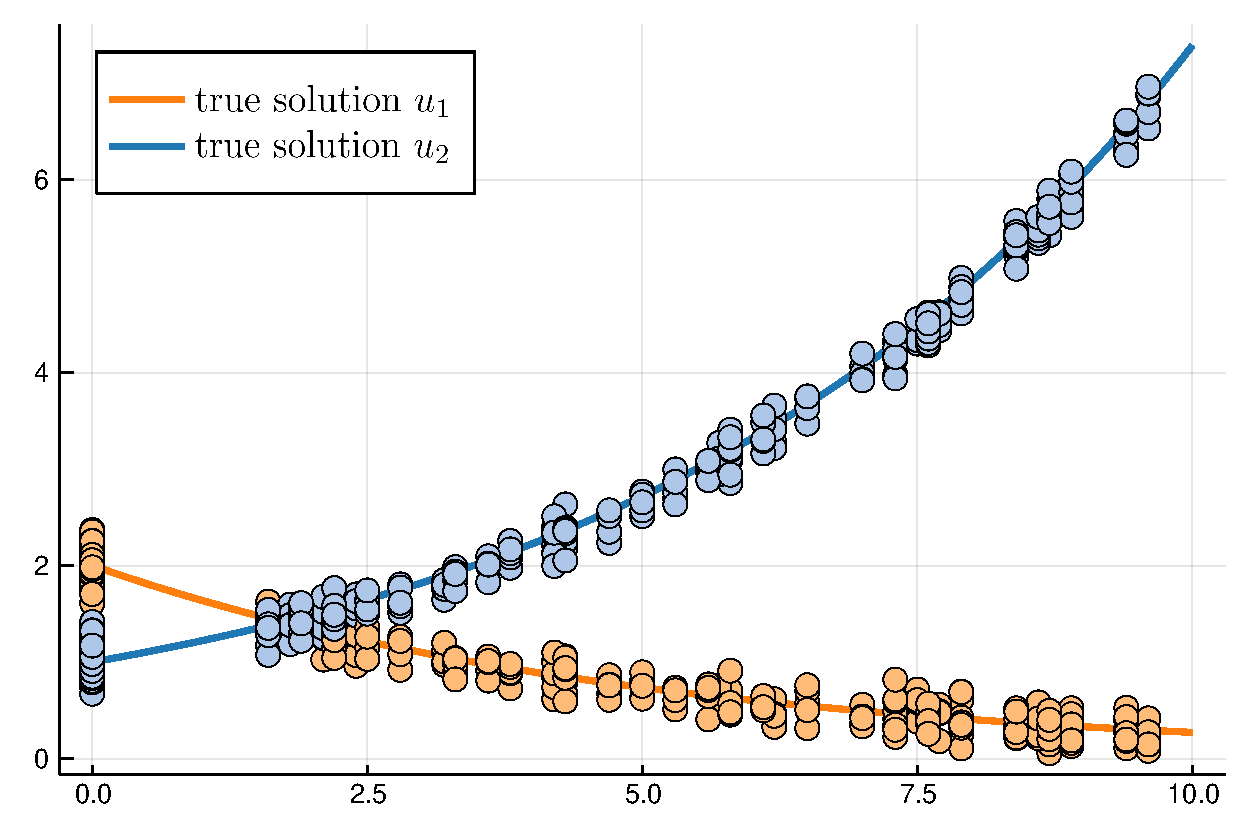
\includegraphics[width=\linewidth]{data_true_solution_2_2ps_linear.pdf}
	\end{minipage}\begin{minipage}{.5\linewidth}
		\centering
		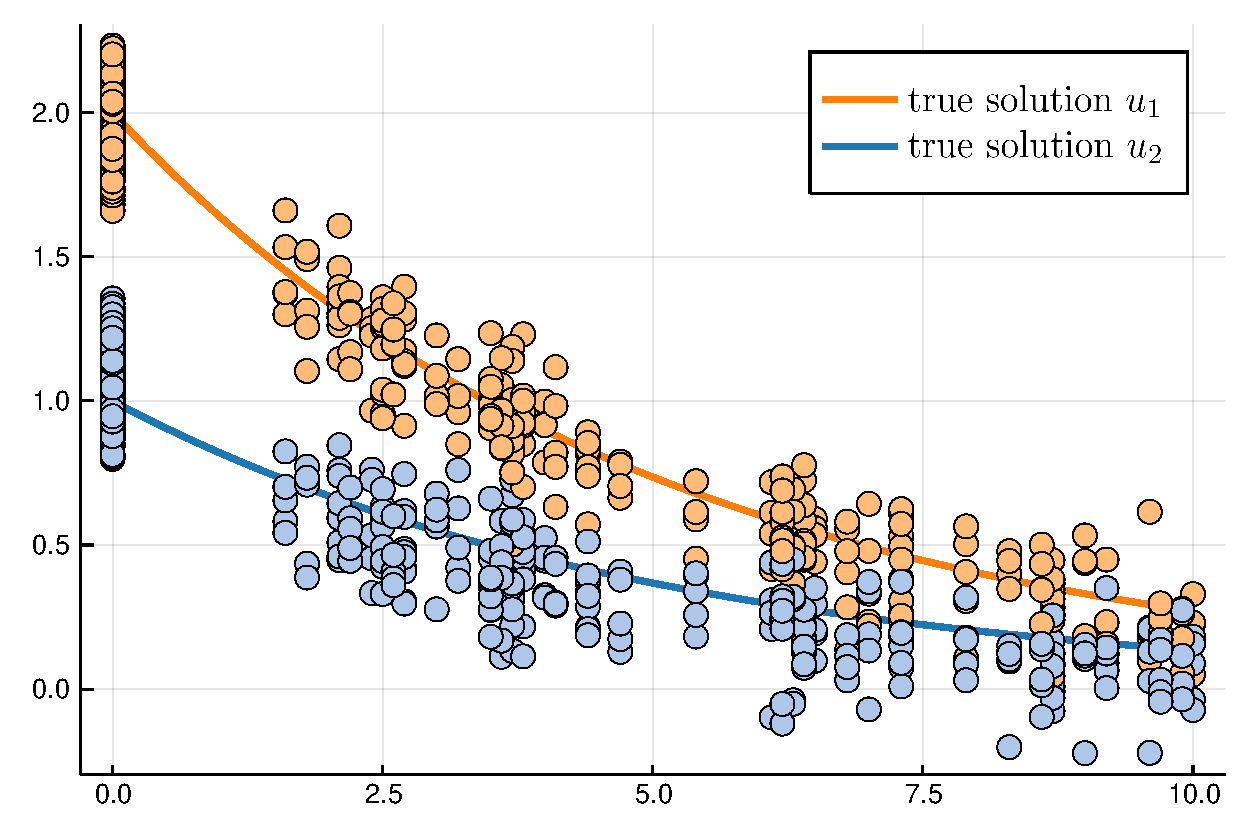
\includegraphics[width=\linewidth]{data_true_solution_1_2ps_linear.pdf}
	\end{minipage}
	\caption{Simulated observations of $100$ individuals ($50$ in each group) at $t_0$ and an individual-specific time point $t_1^i$.}
	\label{fig:data_truesolution_linear2ps}
\end{figure}
To illustrate the structure of each simulated individual's observations, Figure~\ref{fig:20example-ovservations_2ps_linear} exemplarily shows the observations of $20$ simulated study participants on an individual level. Each panel represents one individual, dots represent individual measurements and colors indicate different variables similar to Figure~\ref{fig:exemplary-data} in the introduction. 
\begin{figure}
	\includegraphics[width=\linewidth]{plot_of_10_example_observations_2ps_linear.pdf}
	\caption{Individual-level simulated data structure of $20$ individuals.}
	\label{fig:20example-ovservations_2ps_linear}
\end{figure}

\subsection{Comparison of different simulation scenarios of baseline variables}\label{sec:apps-linear2p-comparisonbaseline}

On the simulated data described in the previous section, the ODE-VAE model is trained as described in Chapter~\ref{chap:methods}, Section~\ref{sec:methods-ODE-VAEtraining}. Specifically, the ODE-net estimates the two non-zero parameters of each of the two ODE systems while the two off-diagonal entries are set to zero, i.e., no interaction is allowed between the components of the ODE solution. Thus, for each individual $i$ the initial value problem 
\begin{equation*}
\begin{split}
	\frac{d}{dt} \mu_i(t) &= \begin{pmatrix} \eta_{i,1} && 0 \\ 0 && \eta_{i,2}	\end{pmatrix} \begin{pmatrix} \mu_{i,1} \\ \mu_{i,2}	\end{pmatrix} (t); \\
	\mu_i(t_0) &= \mu_i\te
\end{split}
\end{equation*}
is solved in latent space at the individual's second measurement time point $t_i^1$ with ODE-net outputs $\eta_{i,1}, \eta_{i,2}$. 

As a first application, I compare the different simulations scenarios of baseline variables described in Algorithms~\ref{algo-simulation-baseline-trueODEparams} and \ref{algo-simulation-baseline-groupinfo}. For the first scenario with the true ODE parameters, I set $\sigma_{\mathrm{info}} = \sigma_{\mathrm{noise}} = 0.1$ and for the second scenario with the group membership, I set $\sigma_{\mathrm{info}} = \sigma_{\mathrm{noise}} = 0.5$, such that for both scenarios, the distributions of noise and the information overlap beyond one standard deviation. In each scenario, I simulate $10$ variables containing the respective baseline information, add $40$ noise variables and train the model for $35$ epochs with the ADAM SGD-optimiser (\cite{Kingma2015}) and a learning rate of $0.0005$. 

Figure~\ref{fig:apps_individual_comparison_tp_gi_2pslinear} depicts the fitted ODE solutions of two individuals both for a model trained with the true ODE parameters and one trained with only the group membership as baseline information. In both scenarios, the model recovers the general structure of the underlying patterns, recognising the distinct upward/downward trends of variables for the two individuals. 
It tends to overestimate the initial value of the first component of the solution and to underestimate it in the second component. For the training with the true ODE parameters, the overestimation of the first component initial value is more pronounced, whereas the underestimation in the second component is smaller than for training with only the group information. 
In both scenarios, the first dimension of the mean obtained directly from the VAE encoder before solving the ODE (blue dots) closely matches the first dimension of the smooth mean obtained as ODE solution (solid blue lines), whereas for the second component, in the second group, the means from the encoder for the second time point (orange dots) match the true ODE solution (dotted orange lines) more closely than the fitted ODE solutions. 
Thus, in general the training strategy 
of matching the means before and after solving the ODE -- to both find a latent representation modelling a smooth trajectory even before solving the ODE and to implicitly condition the ODE solution on the data from the second time point -- works, while there is some variation in whether the focus on matching the ODE solution or matching the data dominates. 
\begin{figure}
	\centering
	\begin{minipage}{\linewidth}
		\begin{minipage}{.5\textwidth}
			\centering				\includegraphics[width=\linewidth]{z_trajectory_plots_2ps_29_tp.pdf}
		\end{minipage}\begin{minipage}{.5\textwidth}
			\centering
			\includegraphics[width=\linewidth]{z_trajectory_plots_2ps_29_gi.pdf}
		\end{minipage}
	\end{minipage}
	\begin{minipage}{\linewidth}
		\begin{minipage}{.5\textwidth}
			\centering
			\includegraphics[width=\linewidth]{z_trajectory_plots_2ps_25_tp.pdf}
		\end{minipage}\begin{minipage}{.5\textwidth}
			\centering
			\includegraphics[width=\linewidth]{z_trajectory_plots_2ps_25_gi.pdf}
		\end{minipage}
	\end{minipage}
\caption{Comparison of fitted ODE solutions of one individual from each group for both scenarios of simulated baseline variables.}
\label{fig:apps_individual_comparison_tp_gi_2pslinear}
\end{figure}

To get a broader overview, the distributions of ODE solutions are compared across the whole dataset. In Figure~\ref{fig:apps_allinds_comparison_tp_gi_2pslinear}, the fitted ODE solutions and encoder means from all individuals of one group are overlayed, and again both groups of underlying development patterns and both scenarios of baseline variables are compared. 

As expected, the results from training with only the group membership as baseline information, representing the more difficult scenario, display a higher variability between individual ODE solutions in both groups. 
In this setting, the model also has greater difficulty matching the upward development in the first group of individuals with the posterior mean before solving the ODE (blue dots). While this trend is underestimated especially for later timepoints ($t>6$) also with the true ODE parameters as baseline information, this becomes more pronounced for training with only the group membership. For both groups and both training scenarios, it seems to be difficult to capture the exponential growth or decay in the latent representation mean before solving the ODE, as can be seen from the blue dots in the panels in the first row and the orange dots in the second row forming a linear rather than an exponential trend. Only the exponential decay of the first ODE component for the first group of individuals is captured in the encoder means (orange dots in the first row).

\begin{figure}
	\centering
	\begin{minipage}{\linewidth}
		\begin{minipage}{.5\textwidth}
			\centering				\includegraphics[width=\linewidth]{all_inds_overlaid_group2_tp_2ps_linear.pdf}
		\end{minipage}\begin{minipage}{.5\textwidth}
			\centering
			\includegraphics[width=\linewidth]{all_inds_overlaid_group2_gi_2ps_linear.pdf}
		\end{minipage}
	\end{minipage}
	\begin{minipage}{\linewidth}
		\begin{minipage}{.5\textwidth}
			\centering
			\includegraphics[width=\linewidth]{all_inds_overlaid_group1_tp_2ps_linear.pdf}
		\end{minipage}\begin{minipage}{.5\textwidth}
			\centering
			\includegraphics[width=\linewidth]{all_inds_overlaid_group1_gi_2ps_linear.pdf}
		\end{minipage}
	\end{minipage}
	\caption{Comparison of fitted ODE solutions of all individual from each group for both scenarios of simulated baseline variables.}
	\label{fig:apps_allinds_comparison_tp_gi_2pslinear}
\end{figure}

\subsection{Comparison of different noise levels in the simulated data}\label{sec:apps-linear2p-comparisonnoise}

To investigate how different levels of noise in the time-dependent variables affect the training of the model, I compare the scenario described in Section~\ref{sec:apps-linear2p-inputdata} to a scenario with the same number of observations from the same underlying ODE solutions, but a higher level of random noise. Specifically, I set $\sigma_{\mathrm{var}} = 0.5$ and $\sigma_{\mathrm{ind}} = 1$. As in Figures~\ref{fig:data_truesolution_linear2ps} and \ref{fig:20example-ovservations_2ps_linear} for the setting with a low level of noise, Figure~\ref{fig:data_truesolution_linear2ps_morenoise} visualises all simulated measurements together with the true ODE solutions while the individual-level structure of $20$ simulated individuals is exemplarily illustrated in Figure~\ref{fig:20example-ovservations_2ps_linear_morenoise}.
\begin{figure}
	\centering
	\begin{minipage}{.5\linewidth}
		\centering
		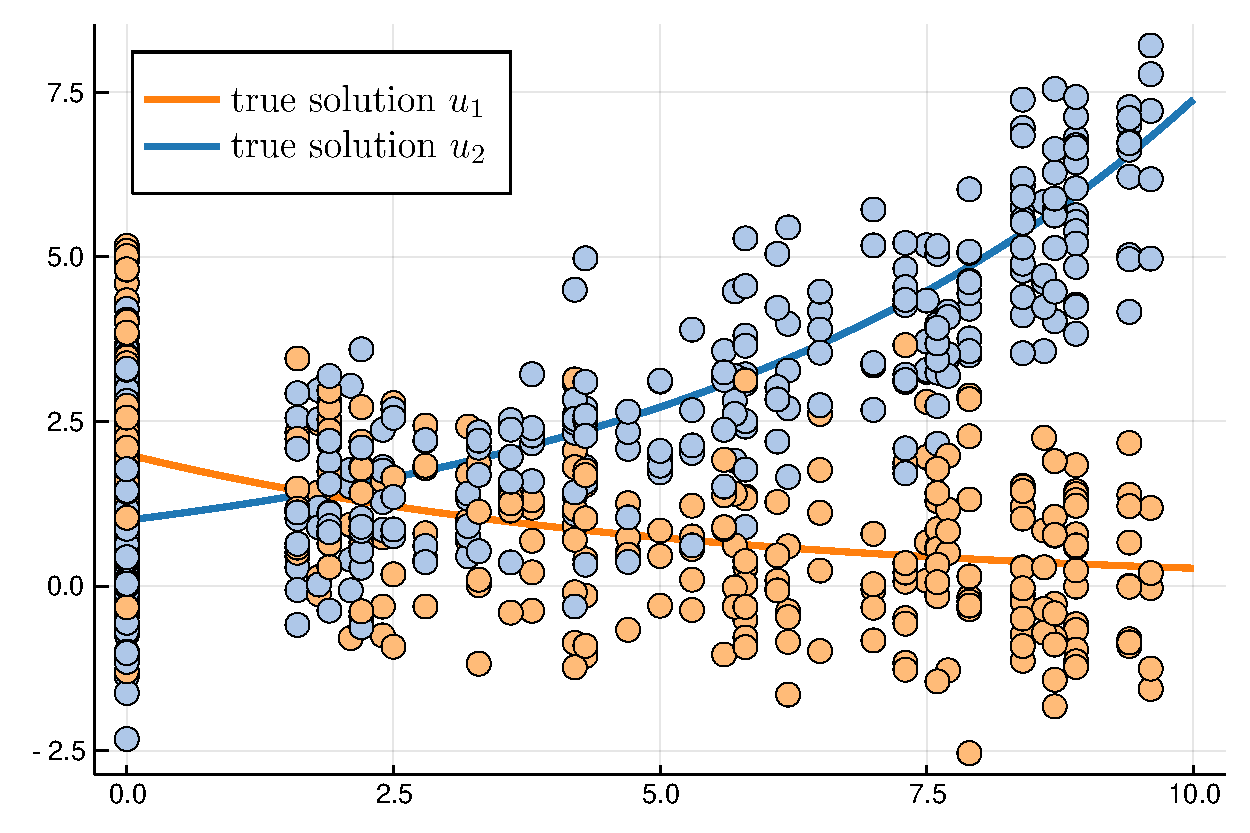
\includegraphics[width=\linewidth]{data_true_solution_2_2ps_linear_morenoise.pdf}
	\end{minipage}\begin{minipage}{.5\linewidth}
		\centering
		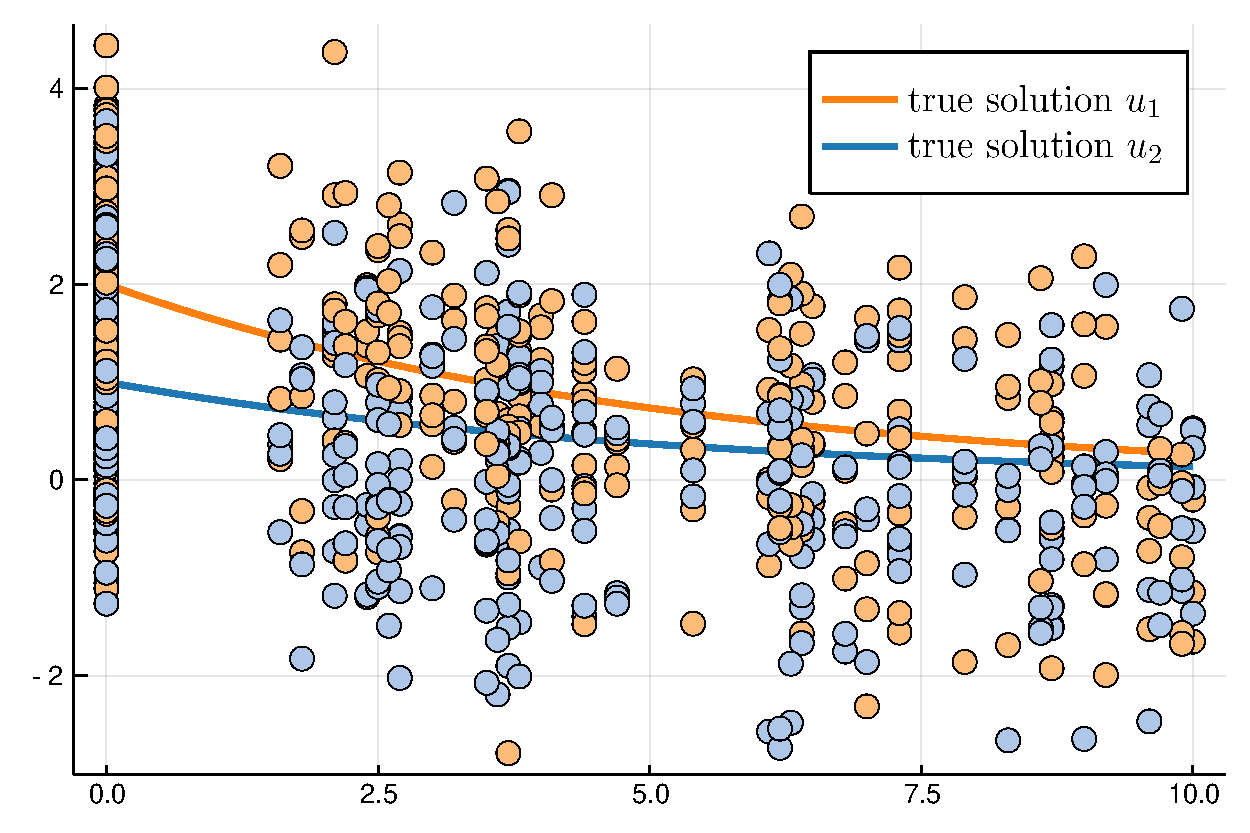
\includegraphics[width=\linewidth]{data_true_solution_1_2ps_linear_morenoise.pdf}
	\end{minipage}
	\caption{Simulated observations of $100$ individuals ($50$ in each group) at $t_0$ and an individual-specific time point $t_1^i$.}
	\label{fig:data_truesolution_linear2ps_morenoise}
\end{figure}
\begin{figure}
	\includegraphics[width=\linewidth]{plot_of_10_example_observations_2ps_linear_morenoise.pdf}
	\caption{Individual-level simulated data structure of $20$ individuals.}
	\label{fig:20example-ovservations_2ps_linear_morenoise}
\end{figure}
For this setting of noisier observations of the true trajectories, I simulate the two versions of baseline variables exactly as in the previous Section~\ref{sec:apps-linear2p-comparisonbaseline} and train the model for $35$ epochs with the ADAM-optimiser and a learning rate of $0.001$.
Figure~\ref{fig:apps_allinds_comparison_morelessnoise_bothgroups_linear} shows a comparison of the results with those from the less noisy setting.
% depicted in Figure~\ref{fig:apps_allinds_comparison_tp_gi_2pslinear}.  
\begin{figure}
	\centering
	\begin{minipage}{\linewidth}
	\includegraphics[width=\linewidth]{comparison_more_less_noise_linear_2ps_group2.pdf}
	\end{minipage}
	\begin{minipage}{\linewidth}
		\includegraphics[width=\linewidth]{comparison_more_less_noise_linear_2ps_group1.pdf}
	\end{minipage}
	\caption{Comparison of fitted ODE solutions of all individual from both groups for both scenarios of simulated baseline variables and two different noise levels.}
	\label{fig:apps_allinds_comparison_morelessnoise_bothgroups_linear}
\end{figure}

First, we can observe that the noisier data setting results in higher variability between fitted ODE solutions (solid lines) as well as the means obtained directly from the encoder (dots) of different individuals. Especially for the second group of individuals (last row), the two components of the mean both from the encoder and as ODE solution are not as distinctly separated. This reflects the setting in the input data: Here, also, the higher noise level results in a substantial overlay of the simulated measurements of both components (see Figure~\ref{fig:data_truesolution_linear2ps_morenoise} and the small figure in the last row of Figure~\ref{fig:apps_allinds_comparison_morelessnoise_bothgroups_linear}). When trained with only the group membership as baseline information, the variability further increases as before, as does the underestimation of the upward trend in the first group of individuals. In the noisier setting, also the downward trend of the first ODE solution component (dotted orange lines) is underestimated in both groups of individuals. 
This is potentially due to the variational posterior being more heavily influenced by the regularising $\mathcal{N}(0,I)$-prior when it gets a weaker input from the data. 

Generally, as the data becomes noisier and the baseline variables become less informative, the latent representations get blurrier, the variability between individuals increases and the two components become less discintly separated, as becomes particularly apparent at the initial value. Nonetheless, despite the substantial level of noise in the data, the model still recovers the general trends and the individual-specific structure of the development patterns. 

\subsection{Training variability}\label{sec:apps-linear2ps-trainingvariability}

As the training objective (\ref{finalELBO}) of the ODE-VAE model represents a non-convex function and hence does not have a unique minimum, the SGD iterative optimisation procedure only approximates a local optimum that depends on the starting point of the algorithm, i.e., the random initialisation of the model weights and biases. To assess the stability with respect to the initialisation, I compare the results across several training runs.

For this application, I employ a moderate level of noise in the time-dependent variables in between the more extreme scenarios compared in the previous Section~\ref{sec:apps-linear2p-comparisonnoise} and set $\sigma_{\mathrm{var}} = 0.1$ and $\sigma_{\mathrm{ind}} = 0.5$. The resulting simulated measurements of the true trajectories are depicted in Figure~\ref{fig:data_truesolution_linear2ps_trainingvariability}.
\begin{figure}
	\centering
	\begin{minipage}{.5\linewidth}
		\centering
		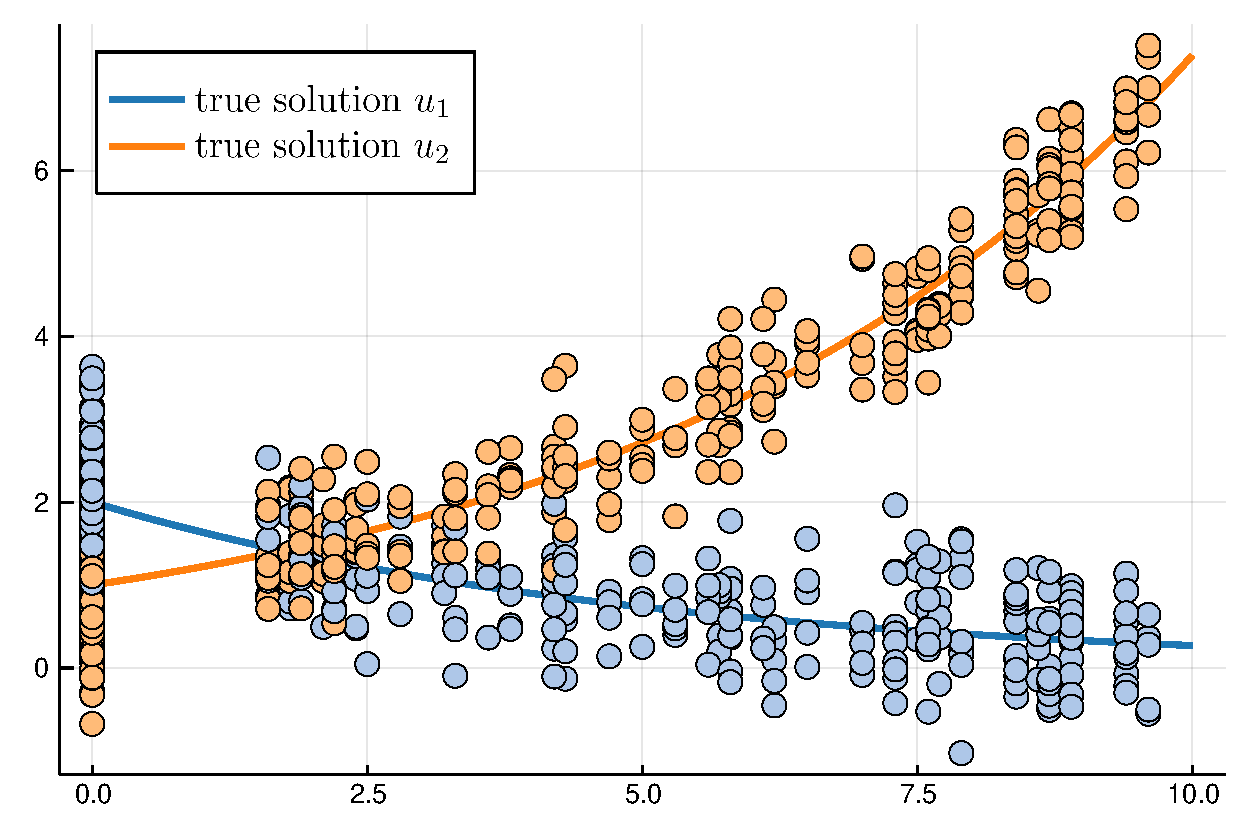
\includegraphics[width=\linewidth]{data_true_solution_2_trainingvariability.pdf}
	\end{minipage}\begin{minipage}{.5\linewidth}
		\centering
		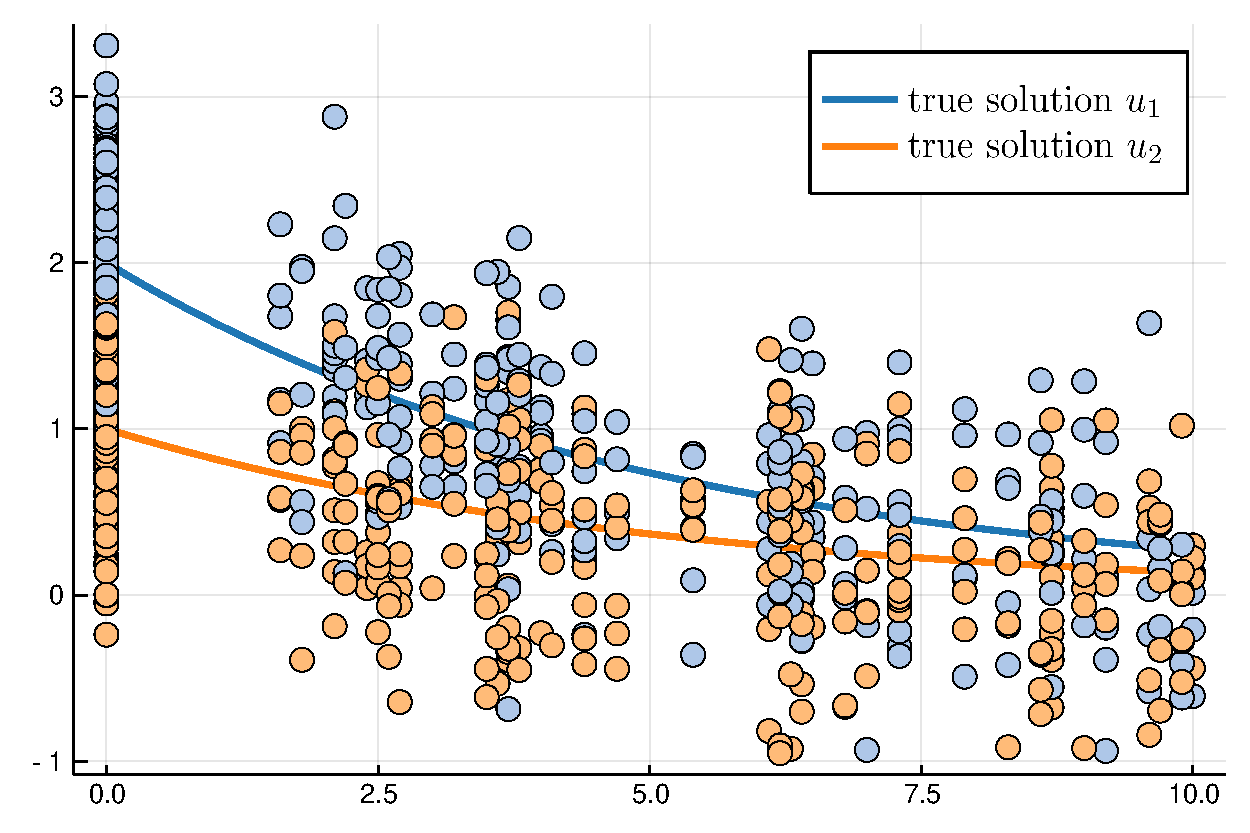
\includegraphics[width=\linewidth]{data_true_solution_1_trainingvariability.pdf}
	\end{minipage}
	\caption{Simulated observations of $100$ individuals ($50$ in each group) at $t_0$ and an individual-specific time point $t_1^i$.}
	\label{fig:data_truesolution_linear2ps_trainingvariability}
\end{figure}

I employ the same two scenarios of simulated baseline variables as before and for each scenario conduct $10$ training runs of the model with different random weight initialisations. In each run, I train the model for $35$ epochs with the ADAM-optimiser and a learning rate of $0.001$. The results are shown in Figure~\ref{fig:apps_training_variability_tp_1} (true ODE parameters as baseline information) and Figure~\ref{fig:apps_training_variability_gi_1} (group membership).
\begin{figure}
	\centering
	\includegraphics[width=\linewidth]{training_variability_bothgroups_trueODEparams_1.pdf}
	\caption{Results of $10$ training runs for model trained with true ODE parameters as baseline information. Each row depicts two training runs and for each run, the two groups of individuals are shown in separate panels.}
	\label{fig:apps_training_variability_tp_1}
\end{figure}

\begin{figure}
	\centering
	\includegraphics[width=\linewidth]{training_variability_bothgroups_groupinfo_1.pdf}
	\caption{Results of $10$ training runs for model trained with group membership as baseline information.}
	\label{fig:apps_training_variability_gi_1}
\end{figure}

Note that the model quite frequently flips one or both components of the initial condition along the $x$-axis. However, the model then also reverses the trend shown by the true trajectories when it flips them to negative values, such that the sign of the corresponding ODE parameter remains the same (a positive parameter in the system defines an upward trend for a positive value of the initial condition and a downward trend for a negative value). The downward trends of the true solution turn into upward trends of the fitted solution when the model flips the initial condition, and vice versa. 
The model thus still infers the distinct group-specific development patterns and assigns to them the correct parameters of the ODE system, it merely embeds the data in a latent representation that flips the signs in one or both dimensions. The neural network architecture defining the model encoder and decoder grants the model freedom to structure its latent representation so that it can potentially flip the signs of the data values in the process of embedding them in latent space and flip them back again in the decoder, and does not enforce or even encourage a latent representation that keeps the signs of the original ODE solution. 
Additionally, the model freedom in structuring the latent space involves the possibility to rescale the input values, such that the entire system is captured in, e.g., a downscaled version. Potentially, this phenomenon may also account for the downscaled representation compared to the original true ODE solutions that we observed in some of the previous applications. 

Regularly, the model also swaps the dimensions, as can be seen from the training runs that appear to have an inverted colour coding: E.g., in the training run depicted in the two right panels in the second row, the orange fitted ODE solutions belonging to the first latent mean component $\mu_1$ match the second component of the ground truth-ODE solution $u_2$ shown in blue and vice versa. This phenomenon can be explained by the fact that the underlying system is symmetric in the two variables and again, the model structure allows it to fit the first five variables of each observation drawn from the first component $u_1$ of the true solution with the second component $\mu_2$ of its latent representation and vice versa. 

In all but one run (the two right panels in the third row in Figures~\ref{fig:apps_training_variability_tp_1} and \ref{fig:apps_training_variability_gi_1}), the model correctly identifies the distinct underlying development patterns in the two groups. 
This run remained the only one where the general structure was not captured by the model, also when I ran $10$ more runs with different initialisations (results not shown). 
The variability across the dataset differs and is generally higher in the means obtained directly from the encoder. Often, the variability in the second group of individuals appears higher, but this is mostly related to the different scale of the $y$-axis in the two groups. Overall, the observations made in Section~\ref{sec:apps-linear2p-comparisonbaseline} apply also to the majority of training runs depicted in Figures~\ref{fig:apps_training_variability_tp_1} and \ref{fig:apps_training_variability_gi_1}, suggesting that while the ODE-VAE model sometimes is subject to substantial variability in the fitted ODE solutions, it is generally capable of stably inferring distinctly parameterised underlying ODE systems.

\section{Non-linear ODE system with two unknown parameters}\label{sec:apps-nonlinear2p}

\subsection{Structure of input data}\label{sec:apps-nonlinear-inputdata}
In the following section, the model is applied on data from a non-linear ODE system. Specifically, I define two distinctly parameterised Lotka-Volterra systems. This two-dimensional non-linear system is used in ecology to describe the dynamics of the interaction of two populations generally denoted the predator and the prey species (\cite[p.~209]{Teschl2012}). The pair of equations is governed by four parameters and has the following form: 
\begin{equation}\label{eq:general-lotka-volterra-system}
	\begin{split}
			\frac{d}{dt} u_1(t) &= \alpha u_1(t) - \beta u_1(t)u_2(t), \\
			\frac{d}{dt} u_2(t) &= \delta u_1(t)u_2(t) - \gamma u_2(t)
	\end{split}
\end{equation}
In the predator-prey model, the first component $u_1$ describes the dynamics of the prey species and the second component $u_2$ describes that of the predator species. The model then assumes that the growth rate of the prey is $\alpha$, if there are no predators present, and that in the presence of predators, the growth rate is reduced proportional to the number of predators, i.e., $\beta$ can be understood as predation rate or meeting rate of prey and predator. Similarly, without prey, i.e., without food supply, the model assumes the number of predators to decay at rate $-\gamma$, and to increase, if there is prey,  proportional to the amount of prey, such that $\delta$ describes the growth rate of the predator in the presence of prey. 

Unlike the linear system employed in the previous Section~\ref{sec:apps-linear2p}, the periodic solutions of the Lotka-Volterra system cannot be calculated analytically in closed form, which means that the solution has to be approximated numerically. 
For more details on the properties of Lotka-Volterra systems, see \cite[pp.~209-215]{Teschl2012}. 

As for the linear system in Section~\ref{sec:apps-linear2p}, I simulate data from two different underlying development patterns given as solutions of the two distinctly parameterised Lotka-Volterra ODE systems defined in Equations (\ref{eq:ODEsystem-nonlinear-1}) and (\ref{eq:ODEsystem-nonlinear-2}) and visualised in Figure~\ref{fig:true_solution_lv}.

\begin{figure}
	\centering
	\begin{minipage}{.5\linewidth}
		\centering
		\includegraphics[width=\linewidth]{true_solution_2_lv.pdf}
		\begin{equation}\label{eq:ODEsystem-nonlinear-1}
		\begin{split}
				\frac{d}{dt}u_1(t) &= 0.5 u_1(t) - u_1(t) u_2(t), \\
				\frac{d}{dt}u_2(t) &= u_1(t) u_2(t) - 2 u_1(t); \\
				u_1(0) &= 2, \\ 
				u_2(0) &= 2
		\end{split}
		\end{equation}
		%\normalsize
	\end{minipage}\begin{minipage}{.5\linewidth}
		\centering
		\includegraphics[width=\linewidth]{true_solution_1_lv.pdf}
		\begin{equation}\label{eq:ODEsystem-nonlinear-2}
		\begin{split}
				\frac{d}{dt}u_1(t) &= u_1(t) - u_1(t) u_2(t), \\
				\frac{d}{dt}u_2(t) &= u_1(t) u_2(t) - 0.5 u_1(t); \\
				u_1(0) &= 2, \\ 
				u_2(0) &= 2 
		\end{split}
		\end{equation}
		%\normalsize
	\end{minipage}
	\caption{True underlying development patterns characterised as solutions of two-dimensional Lotka-Volterra ODE systems.}
	\label{fig:true_solution_lv}
\end{figure}

As described in Algorithm~\ref{algo-simulation-time-dependent}, observations are simulated by adding random noise to values from these true trajectories. 
To account for the higher complexity of the true system, observations of $200$ individuals are generated in this application, such that the randomly drawn second measurement time points more densely cover the entire trajectory. Thus, the model gets observations from all different sections of the true underlying patterns (e.g., observations from the peak at the beginning of the time interval in the second ODE component of the second system, and the upward trend at the end of the time interval). 

Consequently, I generate observations of $100$ individuals in each of the two groups, and again generate observations of $10$ variables by adding variable-specific and the individual-specific measurement errors to $5$ values from each of the two ODE solution components both at the initial time point $t_0 = 0$ and an individual-specific second time point $t_1^i$. 
To optimally observe all parts of the trajectory and cover the entire time interval, I sample the second measurement time points uniformly from the interval $[0,10]$.
In all applications of this section, I set $\sigma_{\mathrm{var}} = \sigma_{\mathrm{ind}} = 0.1$. Figure~\ref{fig:data_truesolution_lv} visualises all simulated observations together with the true ODE solutions.
\begin{figure}
	\centering
	\begin{minipage}{.5\linewidth}
		\centering
		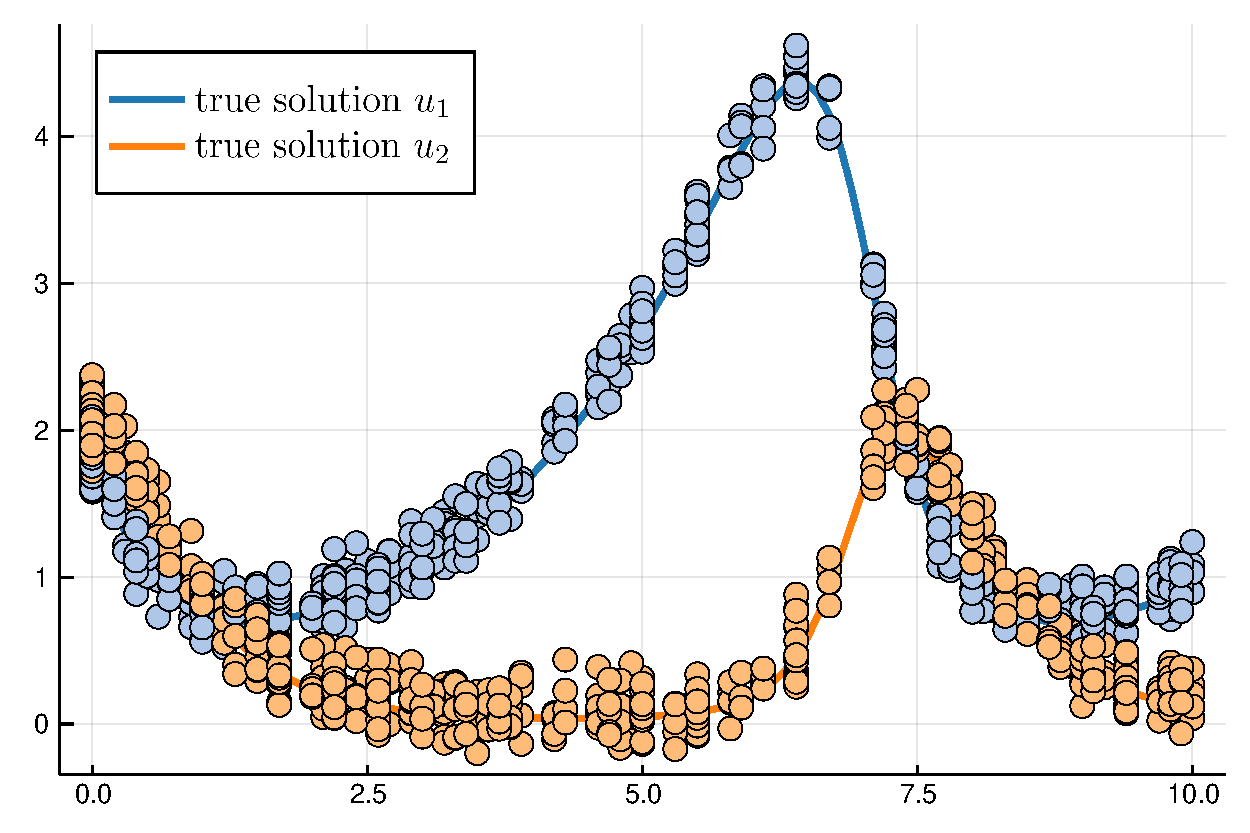
\includegraphics[width=\linewidth]{data_true_solution_2_lv.pdf}
	\end{minipage}\begin{minipage}{.5\linewidth}
		\centering
		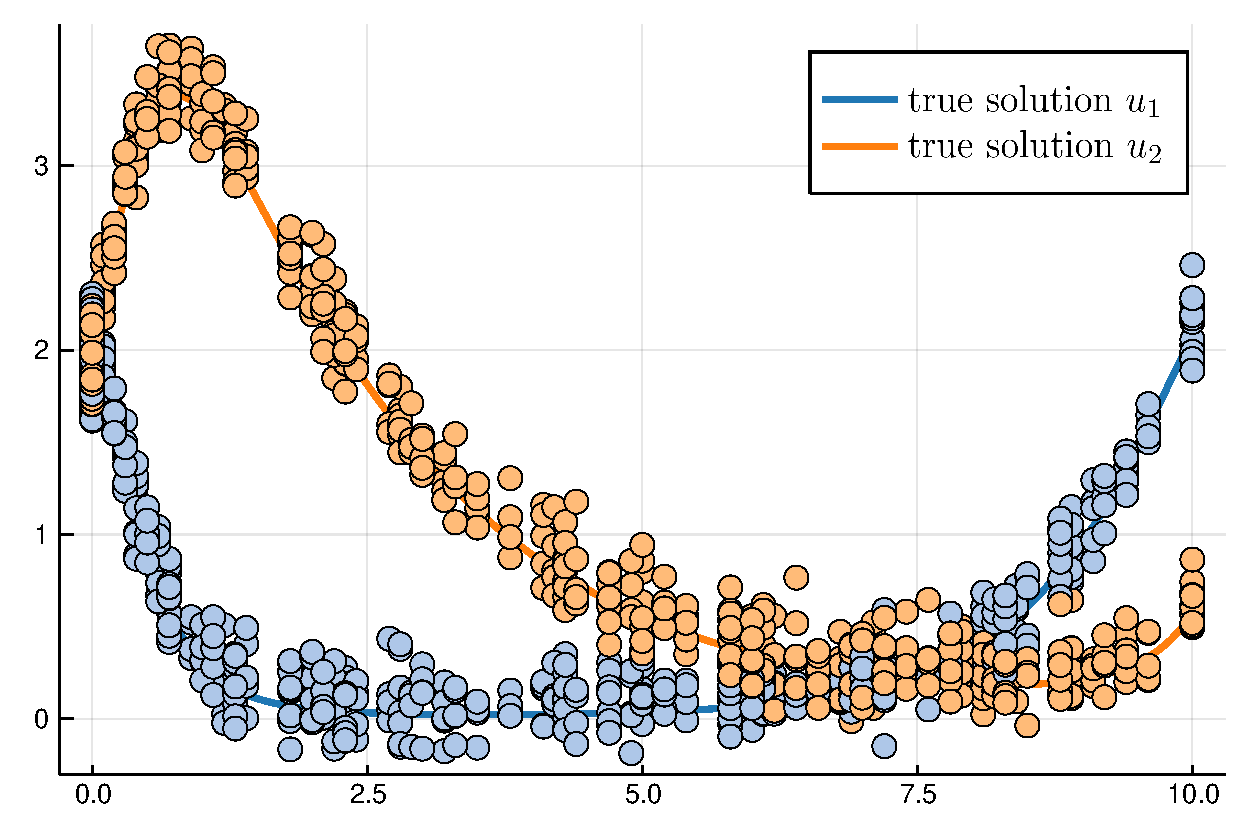
\includegraphics[width=\linewidth]{data_true_solution_1_lv.pdf}
	\end{minipage}
	\caption{Simulated observations of $200$ individuals ($100$ in each group) at $t_0$ and an individual-specific time point $t_1^i$.}
	\label{fig:data_truesolution_lv}
\end{figure}

\subsection{Individual fitted ODE solutions}\label{sec:apps-nonlinear2p-individualresults}

On these simulated data, the ODE-VAE model is trained to estimate the two parameters that differ between the two ODE systems, i.e., the parameters $\beta$ and $\delta$ from (\ref{eq:general-lotka-volterra-system}) describing the interaction of the two components are set to the true value of $1$ and the model learns the two other parameters $\alpha$ and $\gamma$. Thus, for each individual $i$, the initial value problem 
	\begin{equation*}
		\begin{split}
			\frac{d}{dt}\mu_1(t) &= \eta_{i,1} \mu_1(t) - \mu_1(t) \mu_2(t), \\
			\frac{d}{dt}\mu_2(t) &= \mu_1(t) \mu_2(t) - \eta_{i,2} \mu_1(t); \\
			\mu_{i}(t_0) &= \mu_{i}\tn 
\end{split}
\end{equation*}
is solved in latent space at the individual's second measurement time point $t_i^1$ with the ODE-net outputs $\eta_{i,1}, \eta_{i,2}$. 

In this setting, we first look at fitted ODE solutions for selected individuals and compare the two groups of underlying development patterns. For this application, I simulate baseline variables based on the true ODE parameters as in Algorithm~\ref{algo-simulation-baseline-trueODEparams} and set $\sigma_{\mathrm{info}} = \sigma_{\mathrm{noise}} = 0.5$ and $q_{\mathrm{info}}= 30$, i.e., simulate $30$ variables containing the respective baseline information and add $20$ noise variables. Then, I train the model for $40$ epochs with the ADAM SGD-optimiser and a learning rate of $0.0001$. 
\begin{figure}
	\centering
	\begin{minipage}{\linewidth}
		\begin{minipage}{.5\textwidth}
			\centering				
			\includegraphics[width=\linewidth]{z_trajectory_plots_2ps_lv_1early.pdf}
		\end{minipage}\begin{minipage}{.5\textwidth}
			\centering
			\includegraphics[width=\linewidth]{z_trajectory_plots_2ps_lv_1late.pdf}
		\end{minipage}
	\end{minipage}
	\begin{minipage}{\linewidth}
		\begin{minipage}{.5\textwidth}
			\centering
			\includegraphics[width=\linewidth]{z_trajectory_plots_2ps_lv_2early.pdf}
		\end{minipage}\begin{minipage}{.5\textwidth}
			\centering
			\includegraphics[width=\linewidth]{z_trajectory_plots_2ps_lv_2late.pdf}
		\end{minipage}
	\end{minipage}
	\caption{Fitted ODE solutions of four individuals with true ODE parameters as baseline information: Two individuals from each group are shown, one with a second measurement time point rather at the beginning of the time interval (left column) and one with a rather late simulated second measurement (right column).}
	\label{fig:apps_individual_solutions_tp_lv}
\end{figure}

Figure~\ref{fig:apps_individual_solutions_tp_lv} shows the fitted ODE solutions of four individuals.
Generally, the model learns the structure of the underlying patterns in both groups. 
It slightly overestimates the initial value of the first component of the solution and slightly underestimates it in the second component. 
Comparable to the linear setting where the model tends to underestimate the upward trend, in this scenario the model also underestimates the high peaks of the first component $u_1$ for the first underlying pattern and of the second component $u_2$ in the second underlying pattern. 
At the peak of the second component in the left panel of the second row, the model has difficulty matching the mean obtained directly from the encoder (orange dot) to the trajectory of the mean obtained from solving the ODE (solid orange line). As in the linear case, this could be explained by the regularising effect of the $\mathcal{N}(0,I)$-prior on the fitted model posterior and the fact that the true trajectory is rather steep around the peak, such that the data from this region is not dense enough to sufficiently encourage the model to move the posterior to more extreme values away from the prior. 
As the encoder part of the VAE outputting the posterior means before solving the ODE has no access to the baseline variables containing information about the true parameters governing the ODE system, this phenomenon is less pronounced for the mean obtained as ODE solution which can be influenced by the baseline information. 

For the individual from the second group with a late second time point (right panel in second row), the mean from the VAE encoder before solving the ODE in the second component (orange dot) more closely matches the true trajectory (dotted orange line) than the fitted ODE solution (solid orange line). This tendency, albeit less evident, can also be observed for the first component of the mean from the VAE encoder in the both individuals from the first group (blue dots in the panels in the first row) and for the individual with a late second time point also in the second component (orange dot in the right panel of the first row). 
Probably related to the rather low level of noise in the simulated data, the model thus tends to fit a more data-oriented representation of the mean before solving the ODE. This gets more difficult if there is no sufficient data, in which case the regularising $\mathcal{N}(0,I)$-prior gains influence, as for the second mean component in the left panel in the second row.  
Generally, also in the non-linear case the basic distinct trends in the developments are captured and reflected by both the ODE solutions and the means from the VAE encoder. 

\subsection{Training with different numbers of informative baseline variables}\label{sec:apps-nonlinear2p-diffbaselinenumbers}
The aim of this section is to investigate the effect of the numbers of infomative and noise variables at $t_0$. To visualise the variability of the results across the entire dataset and to be able to evaluate the effect of more or less informative baseline variables on the overall model performance, I overlay the fitted ODE solutions of all individuals from each of the two groups and their posterior means from the VAE encoder as in Figures~\ref{fig:apps_allinds_comparison_tp_gi_2pslinear} or \ref{fig:apps_allinds_comparison_morelessnoise_bothgroups_linear}. I conduct four training runs with a different number of informative baseline variables with the time-dependent data described in Section~\ref{sec:apps-nonlinear-inputdata} (Figure~\ref{fig:data_truesolution_lv}). Specifically, I set $q_{\mathrm{info}} = 10, 20, 30, 40$ and for each setting, simulate the baseline information based on the true ODE parameters and the noise variables as described in Algorithm~\ref{algo-simulation-baseline-trueODEparams} with $\sigma_{\mathrm{info}} = \sigma_{\mathrm{noise}} = 0.5$. 
I keep all hyperparameters fixed across the four training runs and always start with the same initialisation of the model weights and biases. As in the previous Section~\ref{sec:apps-nonlinear2p-individualresults}, in each setting, the model is trained for $40$ epochs with the ADAM-optimiser and a learning rate of $0.0001$ without individual tuning of hyperparameters.  
Figure~\ref{fig:apps_allindsoverlaid_diffnobaselines} shows the resulting fitted ODE solutions. 
\begin{figure}
	\centering
	\begin{minipage}{\linewidth}
		\begin{minipage}{.5\textwidth}
			\centering				
			\includegraphics[width=\linewidth]{10inforvars_allindsoverlaid_2.pdf}
		\end{minipage}\begin{minipage}{.5\textwidth}
			\centering
			\vspace{4.2pt}
			\includegraphics[width=\linewidth]{10inforvars_allindsoverlaid_1.pdf}
		\end{minipage}
	\end{minipage}
	\begin{minipage}{\linewidth}
		\begin{minipage}{.5\textwidth}
			\centering				
			\includegraphics[width=\linewidth]{20inforvars_allindsoverlaid_2.pdf}
		\end{minipage}\begin{minipage}{.5\textwidth}
			\centering
			\vspace{4.2pt}
			\includegraphics[width=\linewidth]{20inforvars_allindsoverlaid_1.pdf}
		\end{minipage}
	\end{minipage}	
	\begin{minipage}{\linewidth}
		\begin{minipage}{.5\textwidth}
			\centering				
			\includegraphics[width=\linewidth]{30inforvars_allindsoverlaid_2.pdf}
		\end{minipage}\begin{minipage}{.5\textwidth}
			\centering
			\hspace*{4pt}
			\vspace*{4.2pt}
			\includegraphics[width=\linewidth]{30inforvars_allindsoverlaid_1.pdf}
		\end{minipage}
	\end{minipage}
	\begin{minipage}{\linewidth}
		\begin{minipage}{.5\textwidth}
			\centering				
			\includegraphics[width=\linewidth]{40inforvars_allindsoverlaid_2.pdf}
		\end{minipage}\begin{minipage}{.5\textwidth}
			\centering
			\vspace{4.2pt}
			\includegraphics[width=\linewidth]{40inforvars_allindsoverlaid_1.pdf}
		\end{minipage}
	\end{minipage}
	\caption{Comparison of all individuals' fitted ODE solutions for different baseline variables based on the true ODE parameters. One panel shows the solutions of all individuals from one group of underlying development patterns. One row of panels belongs to one training run with the indicated number of informative baseline variables.}
	\label{fig:apps_allindsoverlaid_diffnobaselines}
\end{figure}

In the first two rows corresponding to the training results with $10$ and $20$ baseline variables carrying information about the true ODE parameters, the model has difficulty inferring the distinct group-specific ODE parameters, as the fitted ODE solutions of both groups are more similar than the actual ground-truth trajectories. While the first underlying pattern is essentially recognised by the model, although with substantial variability, the second underlying ground-truth pattern (right column) is not captured well: The peaks that the model generates in the solutions will in fact also appear in the ground truth solution (due to its periodicity), but at a later time point outside the depicted time interval, indicating that the model underestimates the length of the period of the solution and hence does not infer the correct parameters of the system. 

Additionally, in the first two rows, the model again underestimates the peaks both of the first solution component for the first group of individuals (left column) and of the second solution component in the second group of individuals (right column). With $20$ baseline variables, the model matches the peaks a bit better, reinforcing our previous observation that a lower level of noise helps the model to fit a posterior closer to the data and further away from the $\mathcal{N}(0,I)$-prior.  

Interestingly, in these first two scenarios, the means from the VAE encoder before solving the ODE actually describe the ground truth trajectories better than the fitted ODE solutions and, unlike them, do reflect the different underlying development patterns in the data. 
With $30$ out of $50$ baseline variables carrying information, the model also recovers the second underlying pattern in the fitted ODE solutions. The variability between individuals in both groups is strongly reduced in comparison to the setting with only $10$ informative baseline variables. There is also less variability in the means from the encoder and they better match the ODE solution, although the improvement in performance with respect to the means from the encoder is not as pronounced as for the fitted ODE solutions. 
This is hardly surprising as the VAE encoder is not directly influenced by the baseline information and hence not as sensitive to a higher level of noise in them as the fitted ODE solutions that depend directly on the ODE parameters inferred from the baseline variables. Rather, the fact that they do improve at all confirms again that our training objective of bringing these posterior means from before and after solving the ODE together can successfully guide the model towards finding a meaningful, consistent latent representation and ODE parameters that fit the data.

This becomes evident particularly in the second group of individuals (right column): In the first two rows, where the encoder means describe the ground truth trajectories better than the fitted ODE solutions, there is not much change between $10$ and $20$ informative baseline variables. However, for $30$ baseline variables carrying information, the fitted ODE solutions reflect the underlying true pattern, and also the improvement in the fit of the encoder means is larger than before. Both mean representations are subject to a lower level of variability between individuals and in both components, the means from the encoder match both the ground truth and the fitted ODE solutions much better. This implies that more baseline information helps the VAE to find a better fitting ODE system, and a better fitting ODE system in latent space in turn helps the VAE to find a good latent representation that matches such a smooth development according to the ODE system already as direct output of the encoder, even before solving the ODE. 
In the last row corresponding to the results with $40$ informative baseline variables, compared to the results for $30$ informative baseline variables, mainly the variability across the dataset is further reduced. Even in this last setting, however, the model does not fit the peak of the first solution component in the first group of individual (solid blue lines in left panel) perfectly, and the means from the encoder (blue dots) underestimate it more significantly. In the second component, the means from the encoder do not match the ground-truth trajectory exactly, but still reflect the general non-linear structure. 

When performing the same experiments in the second simulation scenario of baseline variables, i.e., with only the information about the group membership (see Algorithm~\ref{algo-simulation-baseline-groupinfo}), I obtained much better fitting ODE solutions for low numbers of informative baseline variables (see Figure~\ref{fig:apps_allindsoverlaid_diffnobaselines_groupinfo}). Even with only $10$ informative baseline variables and despite the generally more difficult scenario of simulated baseline information, the model still clearly distinguishes the two development patterns and fits them with as little variability as in the setting with the true ODE parameters as baseline information and $30$ informative baseline variables. 
A possible explanation for this phenomenon might be that it can be easier for the model to distinguish between two groups if only the group membership is encoded in the baseline information: With the true ODE parameters as information, it has to take an additional step, i.e., it has to both infer the true parameters from the noisy information and then infer from that there are two groups, while with only the group membership, it is easier for the model to infer the general presence of two distinct groups from the data. 
As in the setting shown in Figure~\ref{fig:apps_allindsoverlaid_diffnobaselines_groupinfo}, the variability between individuals further decreases for an increased number of informative variables and the model generally has difficulty matching the means from the encoder and the means after solving the ODE in the regions of high peaks in the data. 

\begin{figure}
	\centering
	\begin{minipage}{\linewidth}
		\begin{minipage}{.5\textwidth}
			\centering				
			\includegraphics[width=\linewidth]{10inforvars_allindsoverlaid_groupinfo_2.pdf}
		\end{minipage}\begin{minipage}{.5\textwidth}
			\centering
			\vspace{4.2pt}
			\includegraphics[width=\linewidth]{10inforvars_allindsoverlaid_groupinfo_1.pdf}
		\end{minipage}
	\end{minipage}
	\begin{minipage}{\linewidth}
		\begin{minipage}{.5\textwidth}
			\centering				
			\includegraphics[width=\linewidth]{20inforvars_allindsoverlaid_groupinfo_2.pdf}
		\end{minipage}\begin{minipage}{.5\textwidth}
			\centering
			\vspace{4pt}			
			\includegraphics[width=\linewidth]{20inforvars_allindsoverlaid_groupinfo_1.pdf}
		\end{minipage}
	\end{minipage}	
	\begin{minipage}{\linewidth}
		\begin{minipage}{.5\textwidth}
			\centering				
			\includegraphics[width=\linewidth]{30inforvars_allindsoverlaid_groupinfo_2.pdf}
		\end{minipage}\begin{minipage}{.5\textwidth}
			\centering
			\hspace*{1pt}
			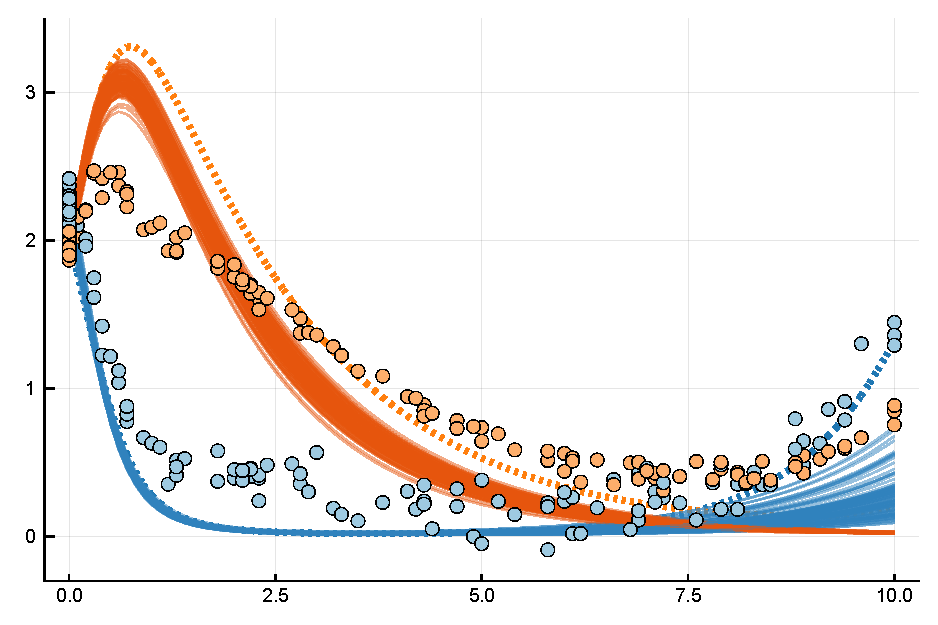
\includegraphics[width=\linewidth]{30inforvars_allindsoverlaid_groupinfo_1.pdf}
		\end{minipage}
	\end{minipage}
	\begin{minipage}{\linewidth}
		\begin{minipage}{.5\textwidth}
			\centering				
			\includegraphics[width=\linewidth]{40inforvars_allindsoverlaid_groupinfo_2.pdf}
		\end{minipage}\begin{minipage}{.5\textwidth}
			\centering
			\vspace{4.5pt}
			\includegraphics[width=\linewidth]{40inforvars_allindsoverlaid_groupinfo_1.pdf}
		\end{minipage}
	\end{minipage}
	\caption{Comparison of all individuals' fitted ODE solutions for different baseline variables based on the group membership. One panel shows the solutions of all individuals from one group of underlying development patterns. One row of panels belongs to one training run with the indicated number of informative baseline variables.}
	\label{fig:apps_allindsoverlaid_diffnobaselines_groupinfo}
\end{figure}

\section{Linear ODE system with four unknown parameters}\label{sec:apps-linear4p}

While the applications presented so far have covered settings where the number of parameters was equal to the number of simulated measurement time points, I now investigate the capability of the ODE-VAE model to fit more parameters in order to model more complex dynamical systems. In the following section, I therefore apply the extension of our training procedure described in Section~\ref{sec:methods-minibatches} and infer batches of individuals with similar trajectories to enrich individual's observations with proxy information at more time points from other individuals in the batch. 

\subsection{Structure of input data}

The model is trained on data from a linear ODE system as in Section~\ref{sec:apps-linear2p} and all four ODE parameters are estimated as outputs of the ODE-net. Again, two distinct underlying development patterns are defined as solutions of the ODE systems in Equations (\ref{eq:ODE-systems-4pslinear-1}) and (\ref{eq:ODE-systems-4pslinear-2}) and visualised in Figure~\ref{fig:apps-true_solution_linear_4ps}, similar to those in Section~\ref{sec:apps-linear2p-inputdata}. 

\begin{figure}
	\centering
	\begin{minipage}{.5\linewidth}
		\centering
		\includegraphics[width=\linewidth]{true_solution_2_4ps_linear.pdf}
		\scriptsize
		\begin{equation}\label{eq:ODE-systems-4pslinear-1}
		\begin{split}
		\frac{d}{dt}\begin{pmatrix} u_1 \\ u_2 \end{pmatrix}(t) &= \begin{pmatrix} -0.2 & 0.1 \\ -0.1 & 0.25 \end{pmatrix} \begin{pmatrix} u_1 \\ u_2 \end{pmatrix}(t); \\
		\begin{pmatrix} u_1 \\ u_2 \end{pmatrix}(0) &= \begin{pmatrix} 4 \\ 2 \end{pmatrix}
		\end{split}
		\end{equation}
		\normalsize
	\end{minipage}\begin{minipage}{.5\linewidth}
		\centering
		\includegraphics[width=\linewidth]{true_solution_1_4ps_linear.pdf}
		\scriptsize		
		\begin{equation}\label{eq:ODE-systems-4pslinear-2}
		\begin{split}
		\frac{d}{dt}\begin{pmatrix} u_1 \\ u_2 \end{pmatrix}(t) &= \begin{pmatrix} -0.2 & 0.1 \\ 0.1 & -0.2 \end{pmatrix} \begin{pmatrix} u_1 \\ u_2 \end{pmatrix}(t); \\
		\begin{pmatrix} u_1 \\ u_2 \end{pmatrix}(0) &= \begin{pmatrix} 4 \\ 2 \end{pmatrix}
		\end{split}
		\end{equation}
		\normalsize
	\end{minipage}
	\caption{True underlying development patterns characterised as solutions of two-dimensional linear ODE systems.}
	\label{fig:apps-true_solution_linear_4ps}
\end{figure}

%As in the previous sections, we simulate our data by drawing measurement points from these true trajectories and adding random noise as described in Algorithm~\ref{algo-simulation-time-dependent}. 
As in Section~\ref{sec:apps-linear2p-inputdata}, I generate observations of $10$ variables for $100$ individuals, $50$ from each of the two groups, by adding variable-specific and the individual-specific measurement errors to $5$ values from each of the two ODE solution components both at the initial time point $t_0 = 0$ and the second time point $t_1^i$ drawn uniformly from the interval $[1.5, 10]$ as in Algorithm~\ref{algo-simulation-time-dependent}. For this setting with four unknown parameters, I set $\sigma_{\mathrm{var}}= 0.1$ and $\sigma_{\mathrm{ind}} = 0.5$. Figure~\ref{fig:apps-data_truesolution_4ps_linear} visualises all simulated observations together with the true ODE solutions.
\begin{figure}
	\centering
	\begin{minipage}{.5\linewidth}
		\centering
		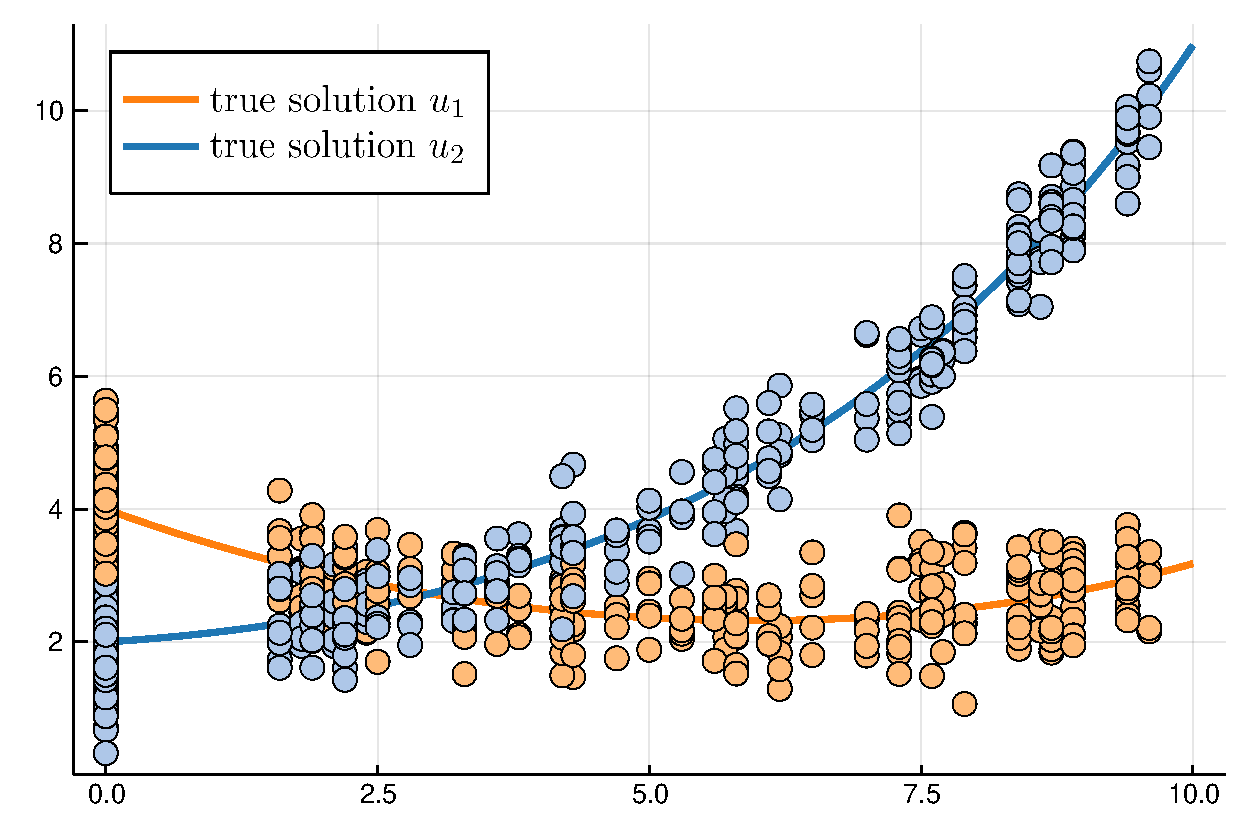
\includegraphics[width=\linewidth]{data_true_solution_2_4ps_linear.pdf}
	\end{minipage}\begin{minipage}{.5\linewidth}
		\centering
		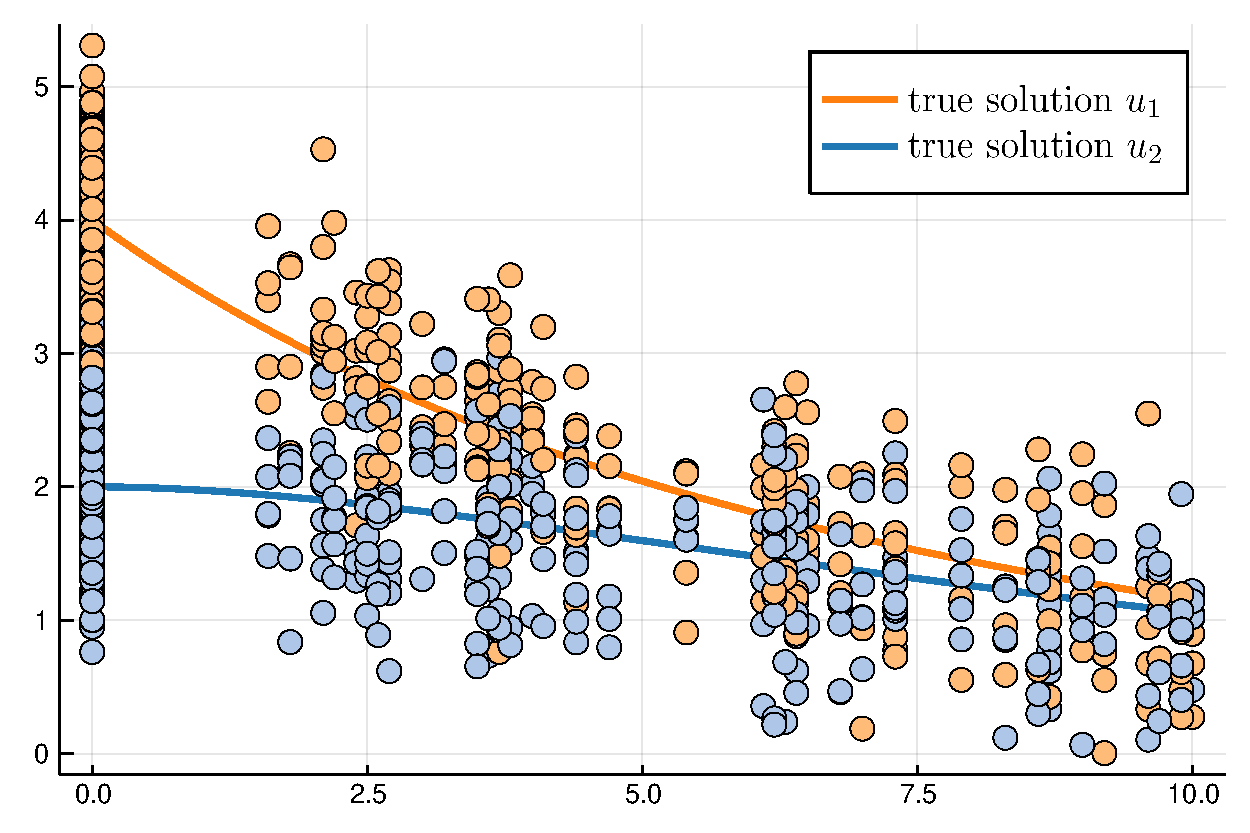
\includegraphics[width=\linewidth]{data_true_solution_1_4ps_linear.pdf}
	\end{minipage}
	\caption{Simulated observations of $100$ individuals ($50$ in each group) at $t_0$ and an individual-specific time point $t_1^i$.}
	\label{fig:apps-data_truesolution_4ps_linear}
\end{figure}

\subsection{Comparison of different simulation scenarios of baseline variables}

On these data, the ODE-VAE model is trained as described in Chapter~\ref{chap:methods}, Section~\ref{sec:methods-minibatches} and Algorithm~\ref{algo-batches}. Specifically, all four parameters of each of the two ODE systems are estimated and in latent space, for each individual $i$ the initial value problem 
\begin{equation*}
	\begin{split}
		\frac{d}{dt} \mu_i(t) &= \begin{pmatrix} \eta_{i,1} && \eta_{i,2} \\ \eta_{i,3} && \eta_{i,4}	\end{pmatrix} \begin{pmatrix} \mu_{i,1} \\ \mu_{i,2}	\end{pmatrix} (t); \\
		\mu_i(t_0) &= \mu_i\te
	\end{split}
\end{equation*}
is solved at the individual's second time point $t_i^1$ with the ODE-net outputs $\eta_{i,1}, \dots, \eta_{i,4}$. 

As in Section~\ref{sec:apps-linear2p-comparisonbaseline}, the different simulations scenarios of baseline variables described in Algorithms~\ref{algo-simulation-baseline-trueODEparams} and \ref{algo-simulation-baseline-groupinfo} are compared. For the first scenario with the true ODE parameters, I set $\sigma_{\mathrm{info}} = \sigma_{\mathrm{noise}} = 0.1$ and for the second scenario with the group membership, I set $\sigma_{\mathrm{info}} = \sigma_{\mathrm{noise}} = 0.5$. In each scenario, I simulate $20$ variables containing the respective baseline information, add $30$ noise variables and train the model for $15$ epochs with the ADAM SGD-optimiser and a learning rate of $0.001$. 

Empirically, I found that for my setting with two distinct underlying patterns, a small batchsize ($b \leq 5$) is insufficient to capture the complete dynamics because it provides too little time points and proxy observations. On the other hand, a large batchsize with respect to the dataset size ($b \gg \frac{n}{10}$) introduces training instability due to too many individuals with different development pattern being grouped together.
Between those extremes, I found the results to be robust against different choices of batchsizes and present in the following only results for a batchsize of $b=10$. 

I also found that the results are stable with respect to different choices of kernel functions, including using equal weights for all individuals in the batch. 
In the more difficult scenario of using only the group membership as baseline information, however, the weighting approach does improve the model performance. Thus, I chose to use the kernel approach for all applications with the tricube function as kernel and a bandwidth of $1$ without tuning this hyperparameter.

Figure~\ref{fig:apps-comparison_tp_gi_individualbatches_linear4ps} compares the ODE solutions of individual minibatches for the two simulation scenarios of baseline variables. 

\begin{figure}
	\includegraphics[width=\linewidth]{comparison_baselinevars_individualsolutions_linear4ps.pdf}
	\caption{Comparison of fitted ODE solutions of selected minibatches for both scenarios of simulated baseline variables. One panel depicts the fitted ODE solutions of all individuals from one batch. Thick, dark lines and dots represent the latent representation means of the reference individual around which the batch was grouped, while lighter, thin lines and dots belong to the other individuals in the batch.}
	\label{fig:apps-comparison_tp_gi_individualbatches_linear4ps}
\end{figure}
Generally, we can see that the second measurement time points of all individuals in the batch do cover the entire time interval, and that all individuals in one batch share a common development trend in both components of the ODE solution.
For training with the group membership as baseline information, we observe the phenomenon mentioned in Section~\ref{sec:apps-linear2ps-trainingvariability} of the inverted signs of the initial condition and the model flipping the first component of the fitted solution at the $x$-axis. In both compared settings, the model again inverts the dimensions, i.e., fits the first component of the true ODE solution with the second component of its latent representation mean and vice versa. 

In the scenario with the true ODE parameters, the fitted ODE solutions show the correct trends of the ground-truth solutions, but, especially in the first component, underestimate the true solution. This is even more pronounced in the first component of the means obtained from the VAE encoder before solving the ODE. However, these means also reflect the true developments with some variability (the apparently higher variability in the second row is due to the different scaling of the axis). When trained with only the group membership as baseline information, the fitted ODE solutions vary more strongly between individuals from the batch, especially in the upper panel. Again, in particular the first component of the fitted ODE solution underestimates the true trend.

Figure~\ref{fig:apps-comparison_tp_gi_allinds_linear4ps} compares the results of all individuals from each of the two groups in the two simulation scenarios of baseline variables by overlaying all individual ODE solutions and encoder means from one group of underlying development patterns in one panel. In general, the variability between individual's solutions from the same group is higher with only the group membership as baseline information. In both scenarios, particularly the upward trend of the second ground-truth ODE solution component is underestimated, while the fitted ODE solutions show that the integrated ODE solving step can partially improve this. 
The variability of the means from the encoder tends to be higher later in the time interval, reflecting the greater uncertainty in the fitted ODE solutions at those later time points. While for the first scenario with the true ODE parameters, the general trends of the trajectories are still distinguishable, they become more and more masked by individual variability in the second scenario.
Our observations are thus generally similar to those for the linear system with only two unknown parameters, although there is more variability and in general a weaker signal present in the application with four unknown parameters. On the other hand, the underlying problem of inferring more parameters than observed time points is much more difficult.

Additionally, I investigated the use of randomly assigned minibatches without inferring individuals' similarity and training without the batches as in the previous sections. Here, I found that without any batches, the model is not able to identify two distinct development patterns at all, and has significantly more difficulty inferring the correct trends of the trajectories with random minibatches. 

Overall, although the results are subject to substantial variation for different initialisations of model weights and biases, the proposed method of training on batches can still enable the achievement of similar results to the two-parameter case in this substantially more difficult setting. 

\begin{figure}
	\includegraphics[width=\linewidth]{comparison_tp_gi_linear_4ps.pdf}
	\caption{Comparison of fitted ODE solutions of all individuals from both groups for both scenarios of simulated baseline variables.}
	\label{fig:apps-comparison_tp_gi_allinds_linear4ps}
\end{figure}